\

We begin our simulations for a variety of starting positions of $N$ ants. For LCS analysis, the starting positions are taken to be the grid points of the grid (so that we can get values of the Finite Time Lyapunov Exponents over the entire grid, more on that later). To make the full grid simulations tenable, we increased the grid spacing $\Delta x$ in that case to 2.5 cm (for a total of 1600 ants).

For generating regular plots, we used a grid spacing of 0.5cm, with $N$ being around 200-300. The positions of the ants in this case are random. In all cases, we observed lane formation almost instantly (within 1000-2000 time steps or equivalently, 10-20 seconds).

We expected to observe ant mill formation, since conditions where ant mills are observed are similar to our grid conditions (ants in a new environment with no prior pheromone deposition) but we didn't, which leads us to believe that ant mill formation is rare, and requires an exact mix of initial conditions that we couldn't replicate in our simulations. In the next section, we analyse the formation and evolution of LCSs in the system created by our model.

\begin{figure}
    \centering
    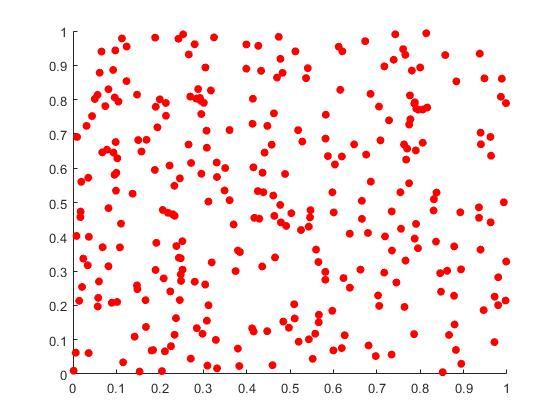
\includegraphics[scale = 0.35]{figures/init_random_pos.jpg}
    \caption{Initial Random Positions for $N = 300$ ants}
    \label{fig:initrandompos}
\end{figure}
\begin{figure}
    \centering
    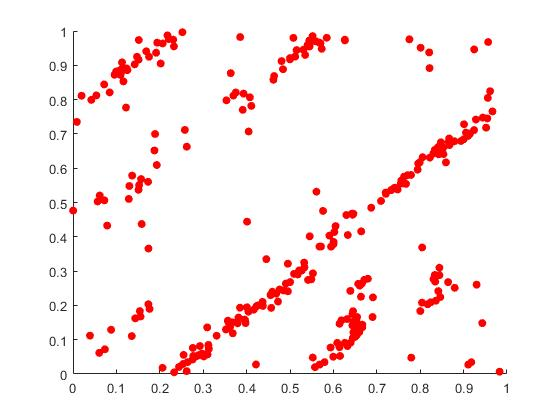
\includegraphics[scale = 0.35]{figures/final_pos_laning.jpg}
    \caption{Final ant positions after $t = 200 s$. Notice the distinctive laning formed as a result of the model}
    \label{fig:finalpos}
\end{figure}
\begin{figure}
    \centering
    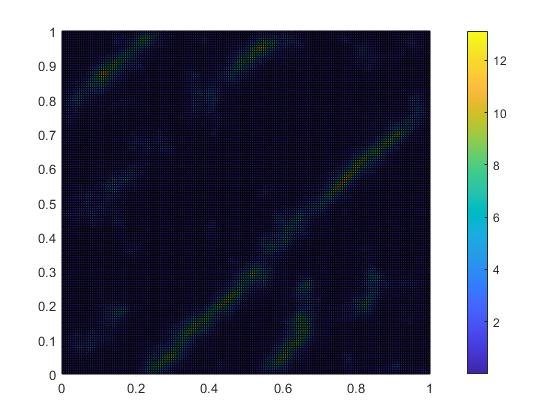
\includegraphics[scale = 0.35]{figures/conc_matrix.jpg}
    \caption{Pheromone concentration after $t = 200s$. There is a high concentration of pheromone deposited along the trails}
    \label{fig:concmatrix}
\end{figure}



